\section{\ApproachName~Overview} \label{sec:overview}

\begin{figure*}[t]
    \centering
    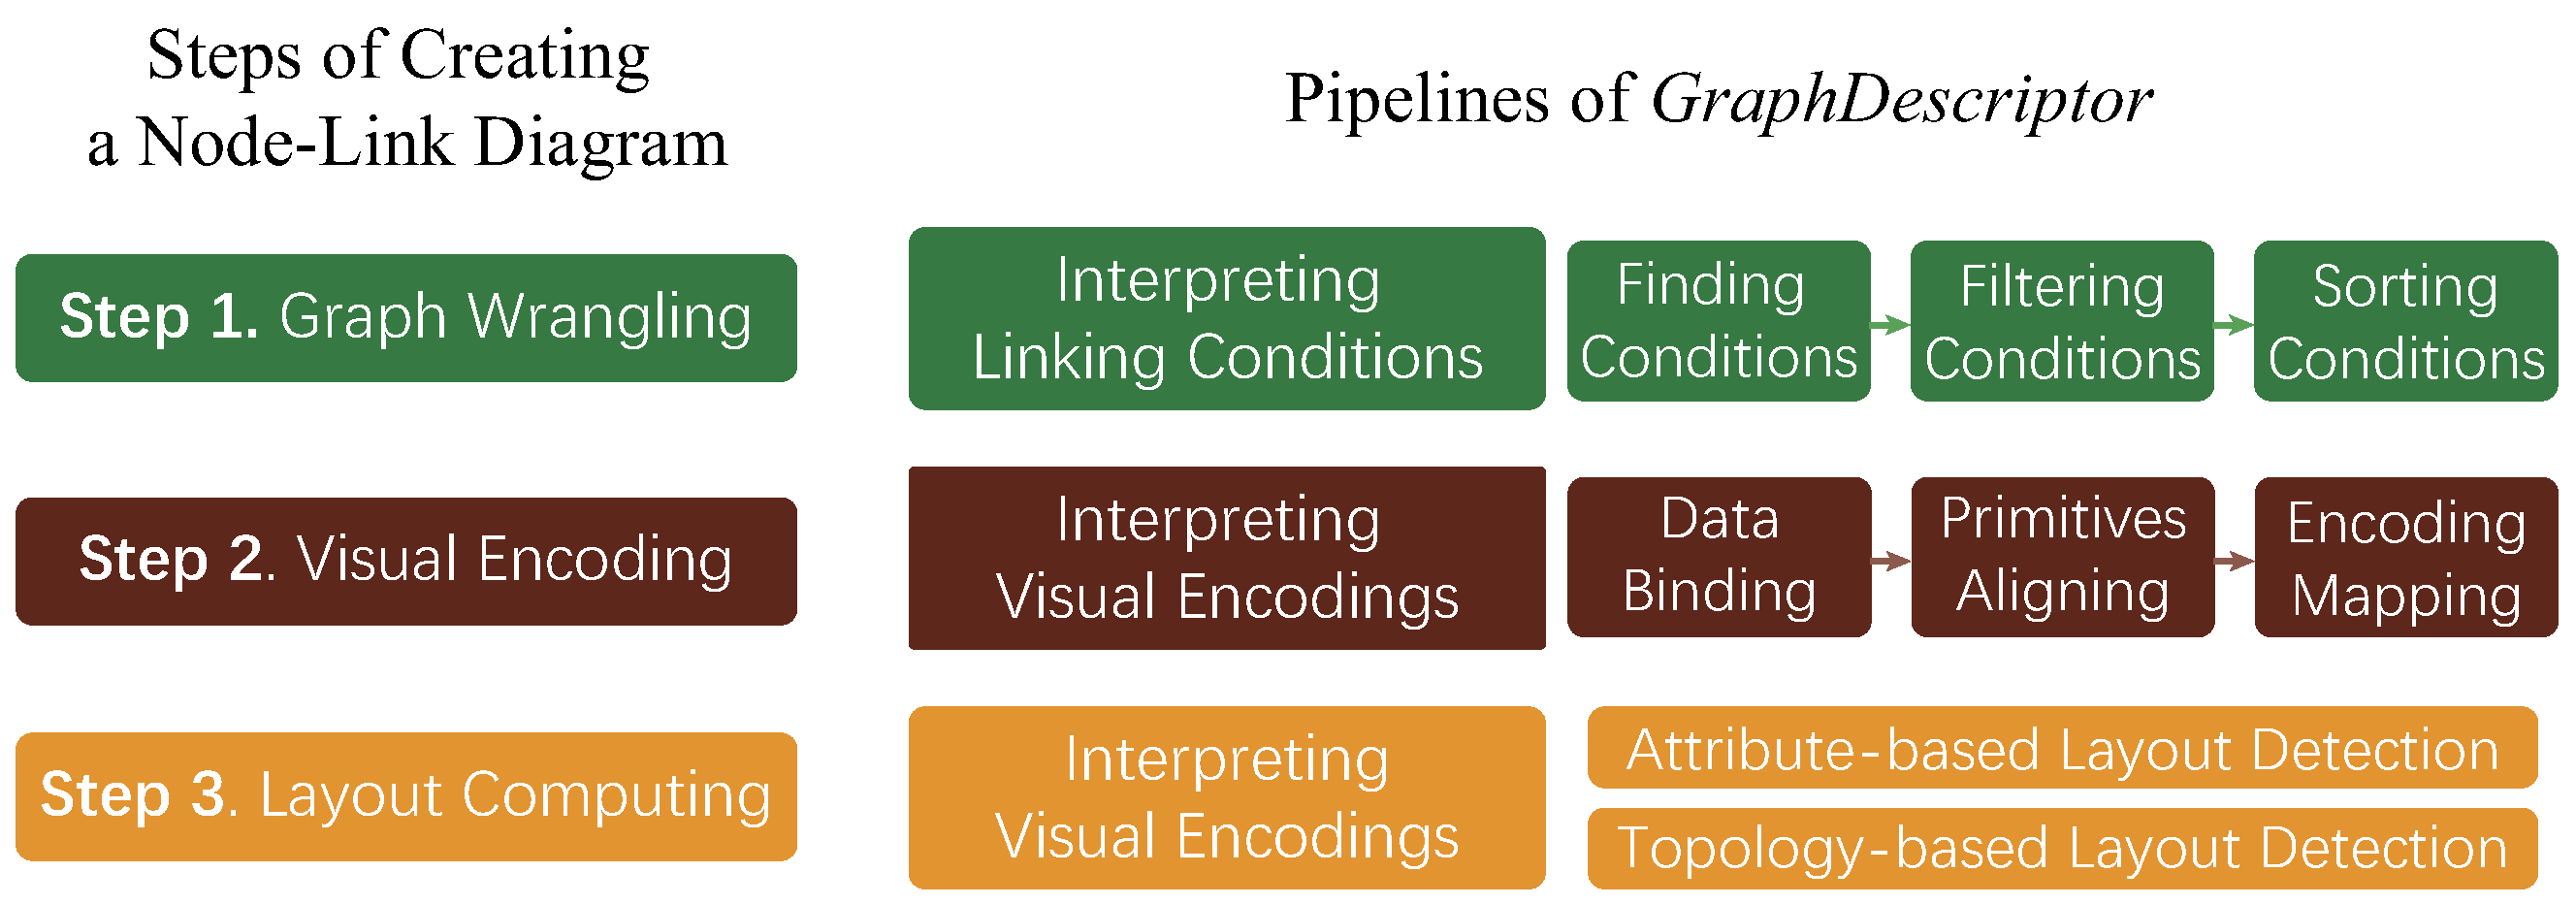
\includegraphics[width=2\columnwidth]{figures/workflow.eps}
    \caption{\ApproachName~consists of two parts: a) GraphExtractor and b) GraphDescriptor. GraphExtractor is used to extracting relevant information from node-link diagram, including meanings of links, visual encodings, and layout type. And GraphDescriptor is used to generating template-based descriptions with interactions. 
    }
    \label{fig:workflow}
\end{figure*}

Following the aforementioned requirements, we propose~\ApproachName~(Figure~\ref{fig:workflow}), an automatic description generation approach, which consists of three information extraction pipelines (GraphExtractor) and a linked description generator (GraphDescriptor). They work together to extract information from node-link diagrams and generate linked descriptions to express the information for end-users.
% inputs here

\subsection{GraphExtractor: Information Extraction Pipelines}

To complete \textbf{\refR{meanings}-\refR{layout-type}}, we design and implement three information extraction pipelines (Figure~\ref{fig:workflow}a):

2) \textbf{Nodes and Links Meanings Extraction Pipeline}. 
To implement \textbf{R1}, we extract the meanings of nodes and links here, to be specific, this pipeline consists of four main steps: 1) extract and summarized node attributes with their value ranges; 2) search candidate link conditions in every pairs of nodes; 3) filter out the wrong conditions; 4) store the remaining conditions with a priority, where a more detailed condition gets a higher ranking.


3) \textbf{Visual Encodings Extraction Pipeline.} 
We extract visual encodings to realize \textbf{R2}. We guide the procedure of extracting visual encodings by three questions: 

\begin{compactenum}[\textbf{Q}1]
    \item \textit{What elements does a node/link consist of in the diagram?} \label{qstn:composition}
    % For example, in Figure~\ref{fig:VisualEncodings}, a node is composed of three rectangles. 
    
    \item \textit{What attributes do elements and their visual channels encode?} 
    \label{qstn:encodings}
    % For example, in Figure~\ref{fig:VisualEncodings}, the left rectangle's height in Node A encodes the first item of the attribute $y$.
    
    \item \textit{Is there a certain type of correlation (positive, negative, or categorical) between attributes and visual channels?}
    \label{qstn:correlation}
    % For example, the greater the degree of the node, the greater the radius of the circle.
\end{compactenum}

Thus, to form the encoding scheme (Figure~\ref{fig:ElementAligning}a), our pipeline extracts 1) mappings between \textbf{data entities} and \textbf{visual elements} and 2) correlations between \textbf{data attributes} and \textbf{visual channels}.

It consists of three steps (Figure~\ref{fig:VisualEncodings}): 1) use \textbf{data binding} to find the mapping between elements and data entities; 2) use \textbf{elements aligning} to align elements according to their \textit{roles}; and 3) use \textbf{encoding mapping} to detect correlations among attributes, elements, and visual channels.

4) \textbf{Layout Type Extraction Pipeline}. 
Based on \textbf{R3}, we propose this pipeline to determine whether the layout is attribute-based or topology-based. This function is handled in two steps: 1) capture the position of each node by computing bounding boxes and 2) determine the layout type by testing the Pearson correlation coefficient.

\subsection{GraphDescriptor: Description Generation Pipeline}
According to \textbf{\refR{text-description}} and \textbf{\refR{interactive-description}}, we propose GraphDescriptor (Figure~\ref{fig:workflow}b) to express the three parts information extracted by GraphExtractor to end-users. This pipeline follows a manner of template-filling, which is a proven method adopt by several description generation approaches~\cite{DBLP:conf/apvis/LiuXHWY20, DBLP:conf/chi/KimHA20}. The sprite of the description is based on the extracted information, although the template bears a resemblance to the skeleton of the description.
We organize the generated descriptions in a pre-set structure to express the extracted information hierarchically. Besides, driven by \textbf{R6}, we link them to their corresponding visual elements to reach an interactive scheme. In this interactive scheme, when users hovering on the descriptions or visual elements, the other element will be highlighted.

